\documentclass{beamer}

\usepackage[utf8]{inputenc}
\usepackage[english]{babel}
\usepackage{amsmath}
\usepackage{hyperref}
\usepackage{color}
\usepackage{pgfplots}
\usepackage{multicol}

\usecolortheme{cormorant}

\title{Oral Progress Report}
\author{Thomas Hill Almeida (21963144)}
\institute{UWA --- OzGrav}
\titlegraphic{
\includegraphics[height=2.5cm]{../resources/UWA.png}}
\date{May 2020}

\pgfplotsset{compat=1.15}

\begin{document}

% Title page
\begin{frame}
    \maketitle
\end{frame}

\begin{frame}{Structure for this report}
    \tableofcontents{}
\end{frame}

\section{Background}
\begin{frame}{Gravitational waves}
    % OzGrav deals with gravitational waves, what are they?
    \begin{itemize}
        \item Predicted to exist in 1915 by the theory of general relativity
        \pause{} \item Shown to exist in 1974 using a binary pair of neutron
            stars
        \pause{} \item Detectors built throughout 2000s failed to reach the
            required sensitivity
        \pause{} \item Increased sensitivity from rebuilds in the 2010s brought
            first direct detection
        \item New detectors still being brought online!
            \begin{itemize}
                \item KAGRA
                \item LIGO India
            \end{itemize}
    \end{itemize}
\end{frame}
\begin{frame}{Pipelines}
    \begin{itemize}
        \item Each detector emits an enormous amount of data
        \pause{} \item Data processing pipelines needed to be developed to
            process and combine outputs
        \pause{} \item Summed Parallel Infinite Impulse Response (SPIIR)
            pipeline
    \end{itemize}
\end{frame}
\begin{frame}{The SPIIR Pipeline}
    \begin{itemize}
        \item IIR filters are typically used in signal processing
        \item Can be used to approximate the shapes of potential gravitational
            waves
        \pause{} \item Later development introduced GPU acceleration
        \item Detection and localization using frequentist coherent search
            added as post-processing step
    \end{itemize}
\end{frame}
\begin{frame}{The SPIIR Pipeline}
    \centering
    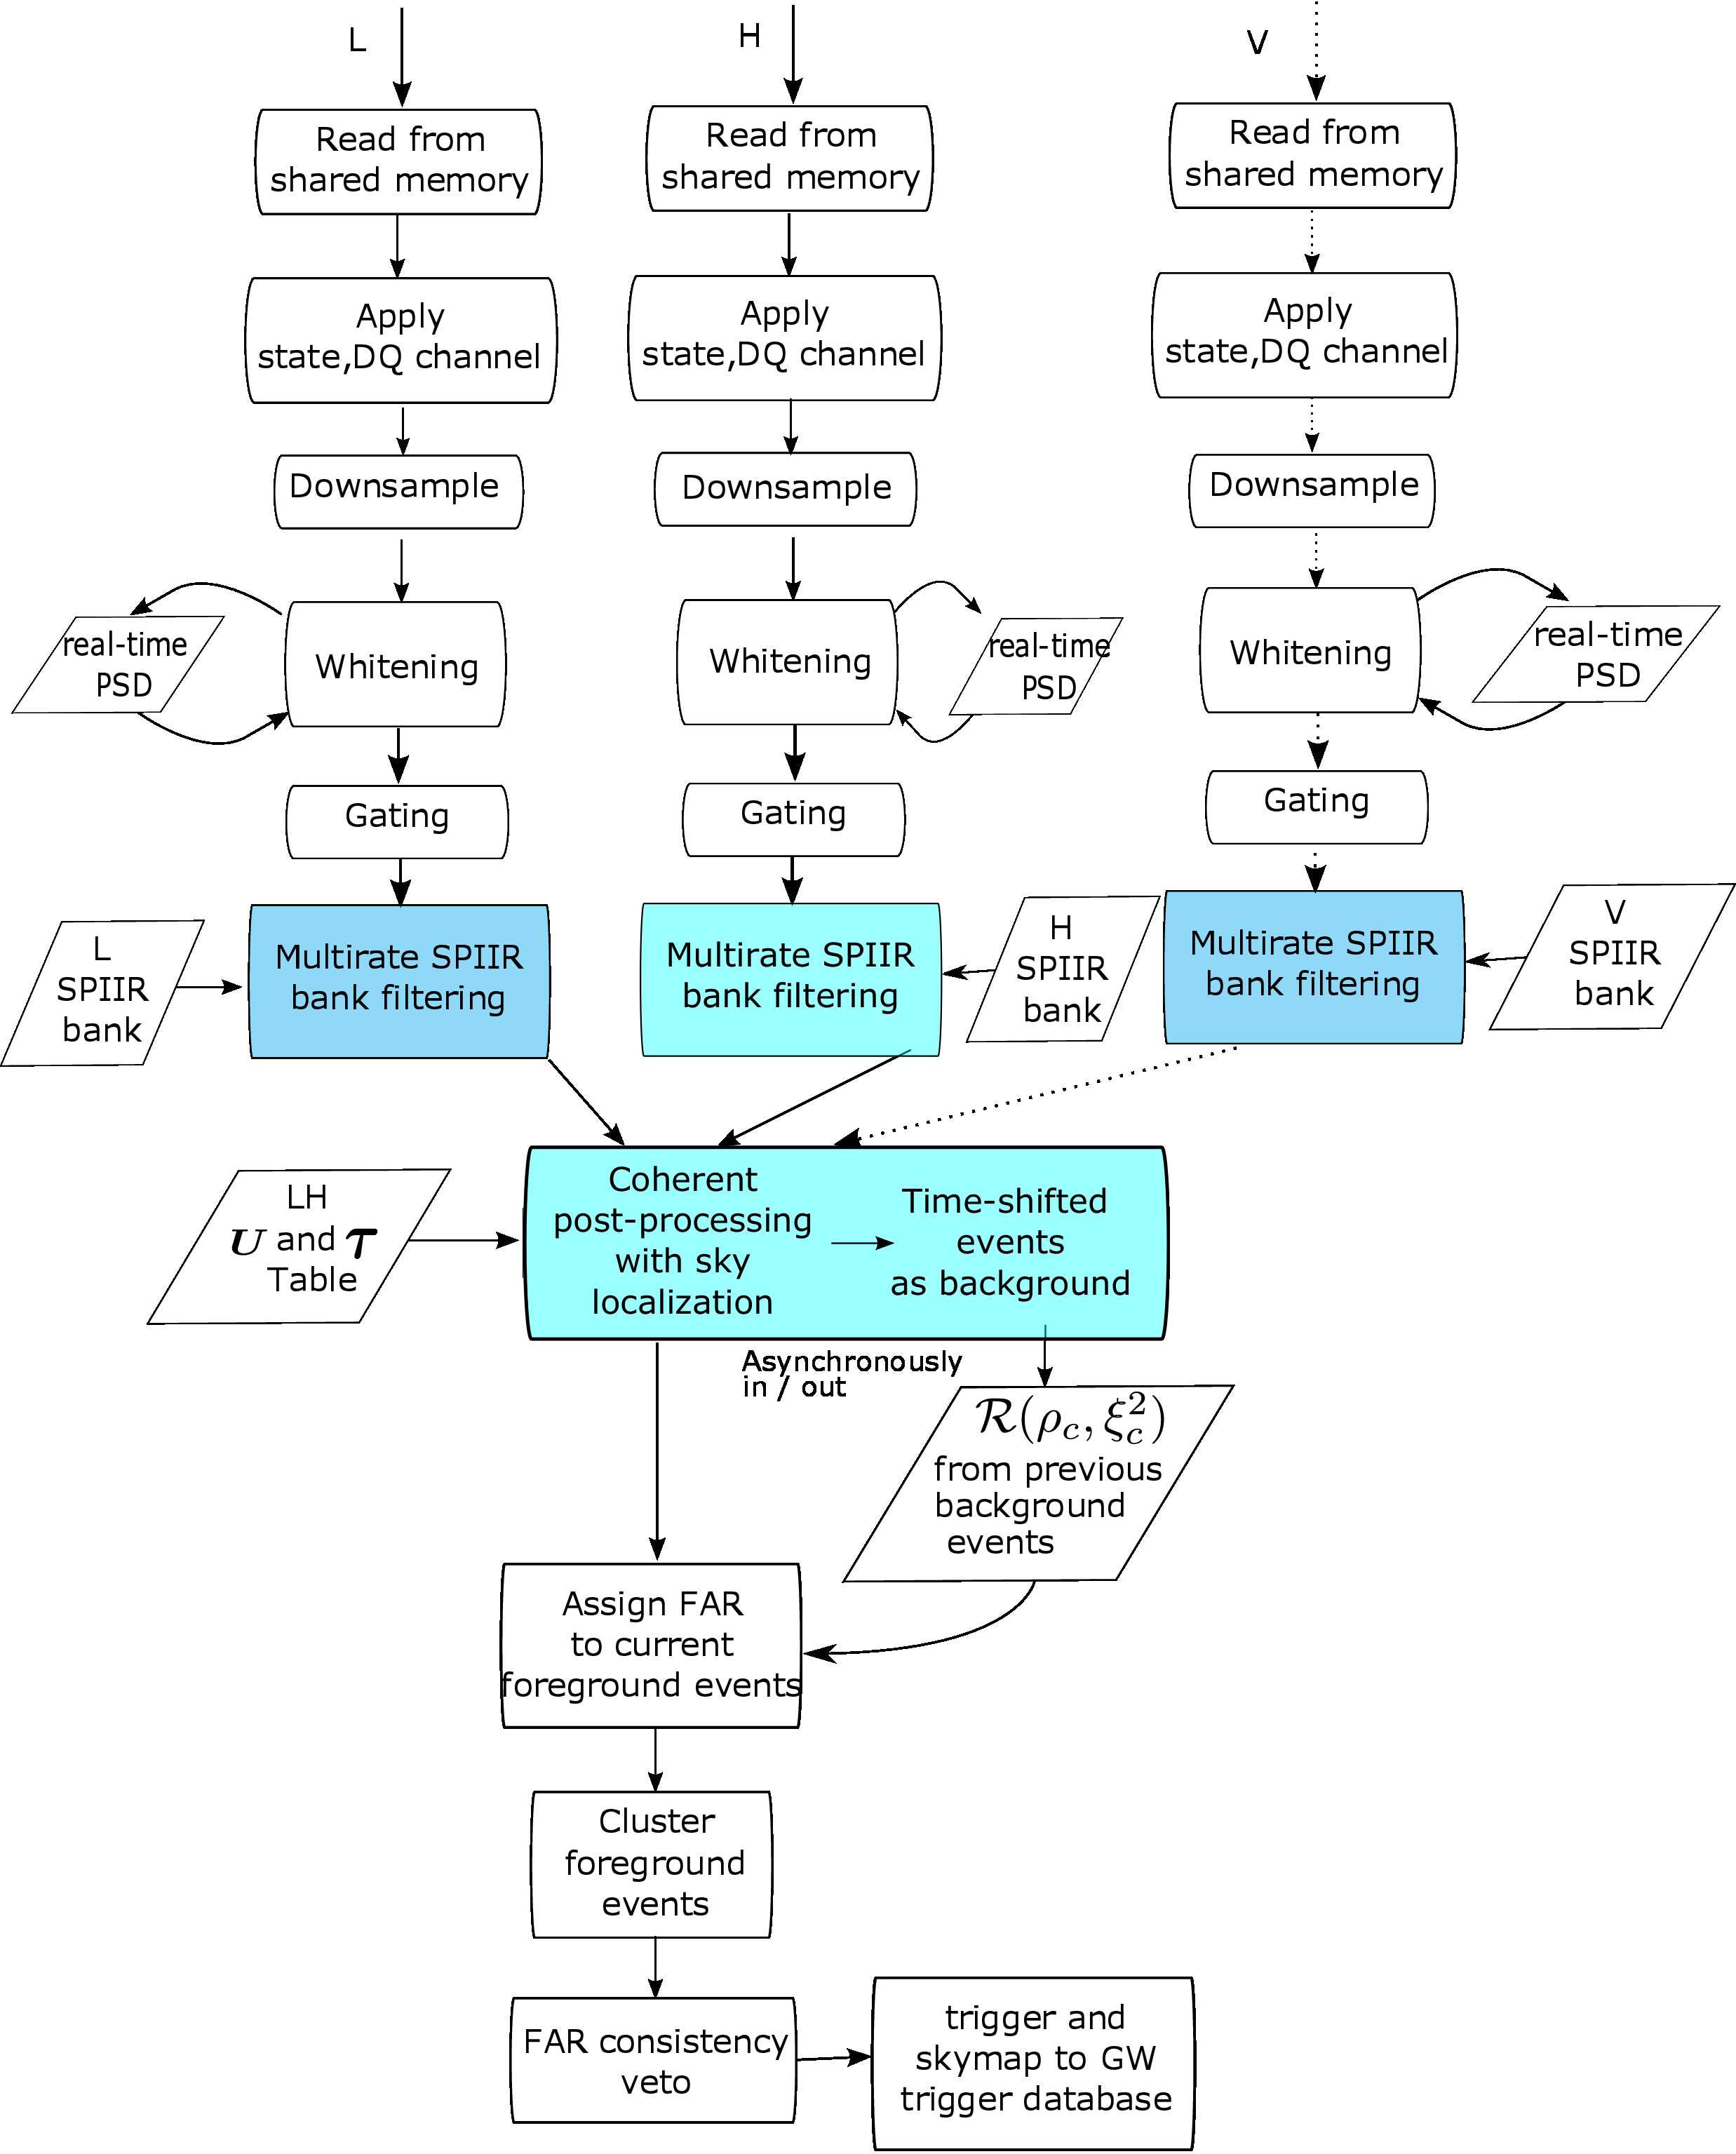
\includegraphics[height=8cm]{online_xdet.jpg}
\end{frame}

\section{Problem Description}
\begin{frame}{Architectural issues}
    \begin{itemize}
        \pause{} \item Maximum of 3 detectors (2 is allowed)
        \pause{} \item Fixed detector ordering
        \pause{} \item All detectors must be used for all parts of
            post-processing
    \end{itemize}
\end{frame}
\begin{frame}{Planned solution}
    \begin{itemize}
        \item Reworked data structures
        \pause{} \item Separation of detection and localization
    \end{itemize}
\end{frame}

\section{Planned method}
\begin{frame}{Planned method}
    \begin{itemize}
        \pause{} \item Develop an understanding of the codebase
            \begin{itemize}
                \pause{} \item What data structures need to be changed?
                \item How are they used?
                \pause{} \item Where can I separate detection and localization?
                \item What are the relevant algorithms?
                \item What's the data flow?
                \pause{} \item Are there any areas for opimization?
            \end{itemize}
        \pause{} \item Refactor the pipeline
        \pause{} \item Measure performance differences
    \end{itemize}
\end{frame}

\section{Progress}
\begin{frame}{Progress}
    \begin{itemize}
        \item Still in analysis phase
        \pause{} \item Developed tools to assist with analysis
        \item Can be useful for other people wishing to analyse similar
            codebases
    \end{itemize}
\end{frame}
\begin{frame}{Progress}
    \centering 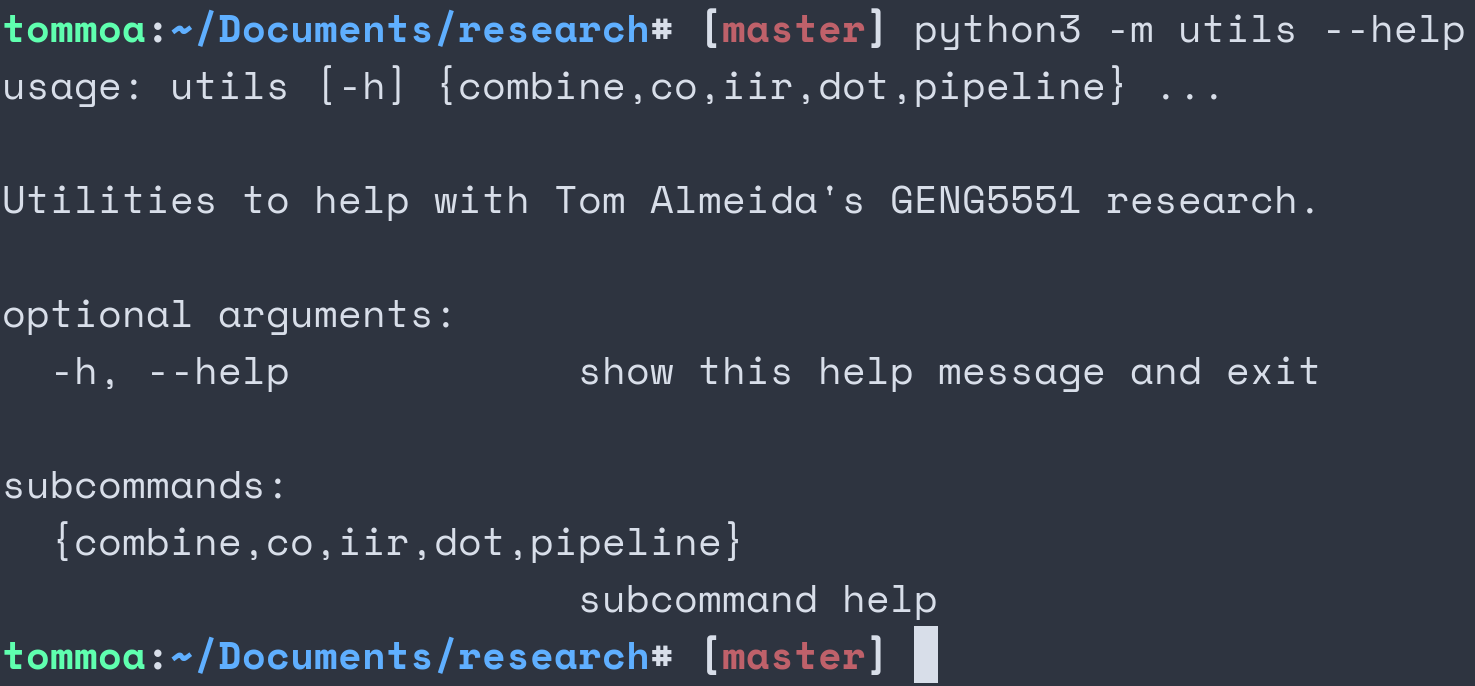
\includegraphics[width=\textwidth]{utils.png}
\end{frame}
\begin{frame}{Progress}
    \centering
    
\includegraphics[width=\textwidth]{callgraph.png}
\end{frame}
\begin{frame}{Progress}
    \begin{itemize}
        \item \texttt{ker\_coh\_skymap}
            \begin{itemize}
                \item \(O(P + C\log{C} + A)\)
                \item Best case could be optimized!
            \end{itemize}
        \item \texttt{ker\_coh\_max\_and\_chisq\_versatile}
            \begin{itemize}
                \item \(O(P(A\log{A} + H(A\log{A} + DA\log{DA})))\)
            \end{itemize}
        \pause{} \item \(A \rightarrow S(D+D^2)\)
        \item \(P \rightarrow\) number of peaks
        \item \(H \rightarrow\) number of hist trials
        \item \(D \rightarrow\) number of detectors
        \item \(S \rightarrow\) number of sky directions
        \item \(C \rightarrow\) size of cohsnr array
        \pause{} \item There are some constant term optimizations to be made!
    \end{itemize}
\end{frame}
\begin{frame}{What's next?}
    \begin{itemize}
        \pause{} \item Analysis of codebase should be finished around the end
            of June
        \pause{} \item Write up of proposed changes by mid-July
        \pause{} \item Start on refactoring mid-July
    \end{itemize}
\end{frame}
\begin{frame}
    \centering
    \begin{block}{\centering Thank you!}
        \centering
        Questions?
    \end{block}
\end{frame}

\end{document}
